\documentclass[aspectratio=43,10pt]{beamer}

% ---------- packages ----------
\usepackage[utf8]{inputenc}
\usepackage{amsmath,amssymb,bm}
\usepackage{graphicx}
\usepackage{booktabs}
\usepackage{array}
\usepackage{tikz}
\usetikzlibrary{arrows.meta,positioning,calc,shapes.geometric}
\usepackage{xcolor}

% ---------- theme / colours (match existing deck) ----------
\usetheme{default}
\definecolor{iitblue}{RGB}{16,48,96}
\definecolor{iitred}{RGB}{200,30,30}

\setbeamercolor{frametitle}{bg=iitblue,fg=white}
\setbeamercolor{footline}{bg=iitblue,fg=white}
\setbeamercolor{title}{fg=white}
\setbeamercolor{structure}{fg=iitblue}
\setbeamercolor{itemize item}{fg=iitblue}
\setbeamercolor{itemize subitem}{fg=iitblue}
\setbeamercolor{itemize subsubitem}{fg=iitblue}
\setbeamercolor{enumerate item}{fg=iitblue}
\setbeamercolor{section in toc}{fg=iitblue}

\setbeamerfont{frametitle}{series=\bfseries,size=\large}
\setbeamerfont{footline}{size=\scriptsize}
\setbeamertemplate{navigation symbols}{}
\setbeamertemplate{itemize item}[circle]
\setbeamertemplate{itemize subitem}[triangle]

% full-width navy frametitle bar (with optional subtitle)
\setbeamertemplate{frametitle}{%
  \nointerlineskip%
  \begin{beamercolorbox}[wd=\paperwidth,sep=0pt]{frametitle}%
    \vskip5pt\hspace{0.35cm}\usebeamerfont{frametitle}\insertframetitle%
    \ifx\insertframesubtitle\empty\else%
      \\\hspace{0.35cm}{\usebeamerfont{framesubtitle}\normalfont\footnotesize\color{white!85!iitblue}\insertframesubtitle}%
    \fi\vskip5pt%
  \end{beamercolorbox}%
}

% centred navy footer
\setbeamertemplate{footline}{%
  \begin{beamercolorbox}[wd=\paperwidth,ht=2.4ex,dp=1.1ex,center]{footline}%
    \usebeamerfont{footline}Department of Chemical Engineering, Indian Institute of Technology, Delhi%
  \end{beamercolorbox}%
}

% ================================================================
\begin{document}

% ----------------------------- Slide 1: Title -----------------------------
\begin{frame}[plain]
  \vspace{0.2cm}
  \begin{beamercolorbox}[wd=\textwidth,sep=10pt,rounded=true,center]{frametitle}
    \usebeamerfont{frametitle}\large
    Study of Magnetic Fluids Showing Negative Viscosity Behavior\\
    Using Lattice Boltzmann Method (LBM)
  \end{beamercolorbox}

  \vfill
  \begin{center}
    
\includegraphics[height=2.6cm]{figs/iitd_logo.png}\\[0.5cm]
    {\small Department of Chemical Engineering\\ Indian Institute of Technology, Delhi}\\[0.35cm]
    {\small\textbf{Submitted by:} Snigdhadyut Dash (2022CH71482)}\\
    {\small\textbf{Supervisor:} Prof.\ Jayati Sarkar}\\[0.45cm]
    {\small\textbf{Mid-Sem Presentation} \quad$\cdot$\quad 24 September 2026}
  \end{center}
  \vfill
\end{frame}

% ----------------------------- Slide 2: Index -----------------------------
\begin{frame}{Outline}
  \vspace{0.3cm}
  \begin{enumerate}
    \item Introduction \& Motivation
    \item Magnetic-fluid specifications
    \item Vector potential --- derivation \& justification
    \item LBM governing equations \& framework
    \item Solver validation --- four tests
    \item Purely magnetically driven flow
    \item Future work, references \& acknowledgments
  \end{enumerate}
\end{frame}

% ============ Section 1 ============
\section{Introduction \& Motivation}

% ----------------------------- Slide 3 -----------------------------
\begin{frame}{Introduction \& Motivation}
  \begin{itemize}
    \item \textbf{Problem Statement:} The microscale coupling between magnetic torque and viscous torque governs how a ferrofluid responds to a field, but it is difficult to predict at the macroscale. Under a suitable oscillating field the effective viscosity can fall, and at strong coupling it becomes negative.
    \item \textbf{Motivation:} A tunable, even negative, apparent viscosity enables valveless micro-pumping, adaptive dampers, and field-guided transport for targeted drug delivery.
    \item \textbf{Objectives:}
      \begin{enumerate}
        \item Establish the 2D/3D torque balances that govern the spin--flow coupling.
        \item Build a robust phase-field MRT Lattice Boltzmann solver for two-fluid magnetic flow.
        \item Validate the solver against analytical limits and the Bacri--Perzynski (1995) benchmark.
      \end{enumerate}
  \end{itemize}
\end{frame}

% ============ Section 2 ============
\section{Magnetic-fluid specifications}

% ----------------------------- Slide 4: Ferrofluid specifications -----------------------------
\begin{frame}{Magnetic-Fluid Specifications}
  \framesubtitle{The benchmark ferrofluid of Bacri, Perzynski \& Shliomis (PRL 75, 1995)}
  \small
  \begin{columns}[T]
    \column{0.52\textwidth}
      \textbf{Physical properties}
      \begin{itemize}
        \item Cobalt-ferrite nanoparticles (Massart synthesis)
        \item Grain magnetization $M_s = 400$~G
        \item Particle size $\sim 10$~nm; anisotropy $K = 2\times10^{6}$~erg/cm$^3$ (rigid dipole)
        \item Carrier: water; volume fraction $\phi = 20\%$
        \item Brownian time $\tau_B \approx 1.6$~ms
        \item Newtonian: $\eta = 77$~cP (zero field) $\to 220$~cP (static $2000$~Oe)
      \end{itemize}
    \column{0.48\textwidth}
      \textbf{Governing balance}
      \[ 6\eta\phi(\bm\omega_p-\bm\Omega)=\bm M\times\bm H \]
      Rotational-viscosity change
      \[ \Delta\eta=\tfrac{3}{2}\,\eta\phi\,\frac{\Omega-\omega_p}{\Omega} \]
      \textbf{Control parameters}
      \[ \xi_0=\frac{M_s V H}{k_BT},\qquad \omega\tau_B \]
  \end{columns}
  \vspace{0.15cm}
  \textbf{Benchmark result:} field frequency alone tunes the viscosity from $220$ down to $50$~cP (over $0$--$700$~Hz), i.e.\ $\Delta\eta$ swings from $+143$ to $-19$~cP. The marginal (zero-viscosity) state is predicted at $\xi_c=126,\ \omega_c\tau_B=20$.
\end{frame}

% ============ Section 3 ============
\section{Vector potential}

% ----------------------------- Slide 5: Vector-potential derivation -----------------------------
\begin{frame}{The Vector-Potential Derivation}
  \small
  Quasi-static Maxwell equations, at every instant:
  \[ \nabla\times\bm H=0,\qquad \nabla\cdot\bm B=0,\qquad \bm B=\mu_0(\bm H+\bm M). \]
  In 2D, a single scalar $A_z$ satisfies the divergence constraint automatically:
  \[ \bm B=\nabla\times(A_z\hat{\bm z})=(\partial_y A_z,\,-\partial_x A_z)\;\Longrightarrow\;\nabla\cdot\bm B\equiv 0. \]
  Imposing $\nabla\times\bm H=0$ gives the governing equation and field recovery:
  \[ \nabla^2 A_z=-\mu_0(\nabla\times\bm M)_z,\qquad \bm H=\bm B/\mu_0-\bm M. \]
  \vspace{-0.15cm}
  \begin{center}\scriptsize
  \begin{tabular}{lll}
    \toprule
     & \textbf{Scalar $\psi$ (old)} & \textbf{Vector $A_z$ (current)} \\
    \midrule
    Poisson equation   & $\nabla^2\psi=\nabla\cdot\bm M$ & $\nabla^2 A_z=-\mu_0(\nabla\times\bm M)_z$\\
    Source             & divergence of $\bm M$ & curl of $\bm M$ \\
    $\nabla\cdot\bm B=0$ & imposed & automatic \\
    Mean field along $x$ & lost (topological) & carried by wall boundary condition \\
    \bottomrule
  \end{tabular}
  \end{center}
  \centering\scriptsize The same Poisson solver is reused; only the source term and the recovery formula change.
\end{frame}

% ----------------------------- Slide 6: Justification -----------------------------
\begin{frame}{Justification: Vector versus Scalar Potential}
  \framesubtitle{Why the scalar potential fails on a periodic channel}
  \small
  \begin{itemize}
    \item \textbf{Scalar choice:} one value per node, $\bm H=-\nabla\psi$, solving
      \[ \nabla^2\psi=\nabla\cdot\bm M . \]
      It is cheap, but it cannot carry a field along the channel.
    \item \textbf{Why it fails:} the channel repeats in $x$, so $\psi$ returns to the same value each period. Its average slope along $x$ is then zero,
      \[ \langle H_x\rangle=-\frac{1}{L}\int_0^L \partial_x\psi\,dx=-\frac{\psi(L,y)-\psi(0,y)}{L}=0, \]
      and the applied field disappears. This is a property of the closed loop, not of static versus oscillating fields.
    \item \textbf{The fix:} build the field from a vector potential $A_z$,
      \[ \bm B=\nabla\times(A_z\hat{\bm z}),\qquad H_x=\tfrac{1}{\mu_0}\,\partial_y A_z . \]
      A steady field along $x$ is stored as a change in $y$ (the walled direction), where no loop closes, so the field is kept.
  \end{itemize}
\end{frame}

% ============ Section 4 ============
\section{LBM framework \& equations}

% ----------------------------- Slide 7: LBM equations -----------------------------
\begin{frame}{LBM Governing Equations (D2Q9)}
  \small
  \textbf{Interface} --- conservative Allen--Cahn ($g$-lattice):
  \[
    g_k^{eq}=w_k\phi\Big[1+\tfrac{\bm c_k\cdot\bm u}{c_s^2}\Big]
      +w_k\tfrac{M_\phi}{c_s^2}\tfrac{4}{D}\phi(1-\phi)\,\bm c_k\cdot\hat{\bm n},\qquad \phi=\textstyle\sum_k g_k .
  \]
  \textbf{Hydrodynamics} --- pressure-based MRT ($f$-lattice):
  \[
    f_k^{eq}=w_k\,p+\rho c_s^2(\Gamma_k-w_k),\qquad \bm F_{tot}=\bm F_s+\bm F_m+\bm F_b .
  \]
  \textbf{Magnetization dynamics} --- MRSh effective-field model:
  \[
    \bm M=\phi M_s L(\xi_e)\hat{\bm e},\qquad
    \frac{d\bm\xi_e}{dt}=\bm\Omega\times\bm\xi_e-\frac{1}{\tau_B}\frac{L}{L'}\!\Big(1-\tfrac{\xi_\parallel}{\xi_e}\Big)\hat{\bm e}+\frac{1}{2\tau_B}\Big(\tfrac{\xi_e}{L}-1\Big)\bm\xi_\perp .
  \]
  \textbf{Magnetostatics} ($h$-lattice) and \textbf{body force}:
  \[
    \nabla^2 A_z=-\mu_0(\nabla\times\bm M)_z,\quad \bm H=\bm B/\mu_0-\bm M,\quad
    \bm F_m=\mu_0(\bm M\cdot\nabla)\bm H+\tfrac12\nabla\times(\mu_0\bm M\times\bm H).
  \]
\end{frame}

% ----------------------------- Slide 8: LBM framework infographic -----------------------------
\begin{frame}{The LBM Framework --- Three Coupled Lattices}
  \centering
  \scriptsize
  \resizebox{0.97\textwidth}{!}{%
  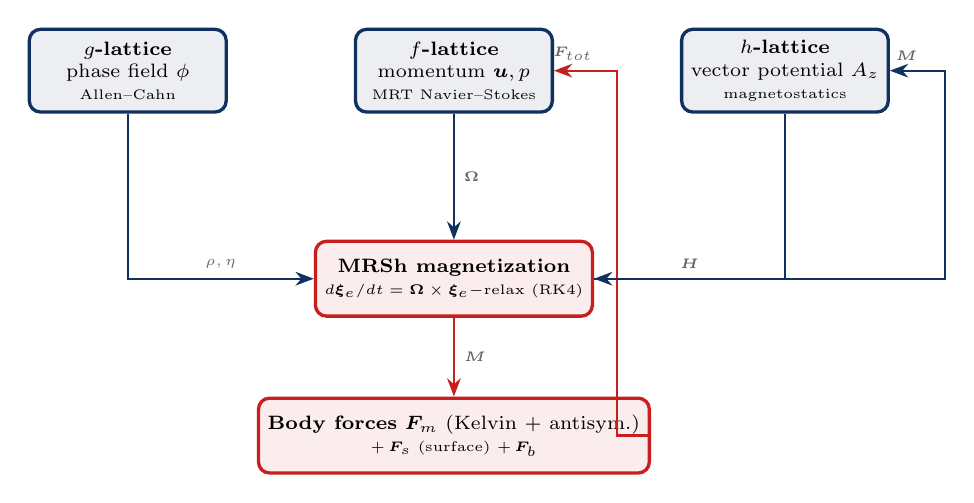
\begin{tikzpicture}[
      >=Stealth, node distance=4mm,
      lat/.style={draw=iitblue,very thick,rounded corners,fill=iitblue!8,
                  align=center,minimum width=2.5cm,minimum height=1.05cm,font=\scriptsize},
      proc/.style={draw=iitred,very thick,rounded corners,fill=iitred!8,
                   align=center,minimum width=2.9cm,minimum height=0.95cm,font=\scriptsize},
      lab/.style={font=\tiny\itshape,text=black!60}]
    \node[lat] (g) {\textbf{$g$-lattice}\\ phase field $\phi$\\ \tiny Allen--Cahn};
    \node[lat,right=1.6cm of g] (f) {\textbf{$f$-lattice}\\ momentum $\bm u,p$\\ \tiny MRT Navier--Stokes};
    \node[lat,right=1.6cm of f] (h) {\textbf{$h$-lattice}\\ vector potential $A_z$\\ \tiny magnetostatics};
    \node[proc,below=1.6cm of f] (m) {\textbf{MRSh magnetization}\\ \tiny $d\bm\xi_e/dt=\bm\Omega\times\bm\xi_e-$relax (RK4)};
    \node[proc,below=1.0cm of m] (F) {\textbf{Body forces} $\bm F_m$ (Kelvin + antisym.)\\ \tiny $+\,\bm F_s$ (surface) $+\,\bm F_b$};

    \coordinate (farA) at ($(h.east)+(0.7,0)$);

    \draw[->,iitblue,thick] (g.south) |- node[lab,pos=0.75,above]{$\rho,\eta$} (m.west);
    \draw[->,iitblue,thick] (f.south) -- node[lab,right]{$\bm\Omega$} (m.north);
    \draw[->,iitblue,thick] (h.south) |- node[lab,pos=0.75,above]{$\bm H$} (m.east);
    \draw[->,iitred,thick] (m.south) -- node[lab,right]{$\bm M$} (F.north);
    \draw[->,iitred,thick] (F.east) -| ($(f.east)+(0.8,0)$) |- node[lab,pos=0.85,above]{$\bm F_{tot}$} (f.east);
    \draw[->,iitblue,thick] (m.east) -| (farA) |- node[lab,pos=0.85,above]{$\bm M$} (h.east);
  \end{tikzpicture}%
  }

  \vspace{0.35cm}
  \normalsize
  \textit{The flow tilts the magnetization; the magnetization sets the body force; the force drives the flow. The three lattices are advanced together every timestep.}
\end{frame}

% ============ Section 5 ============
\section{Solver validation}

% ----------------------------- Slide 9: Base-flow accuracy (Poiseuille) -----------------------------
\begin{frame}{Base-Flow Accuracy --- Poiseuille Profile}
  \framesubtitle{The most basic check: the hydrodynamic solver before any magnetic coupling}
  \begin{columns}[T]
    \column{0.56\textwidth}
      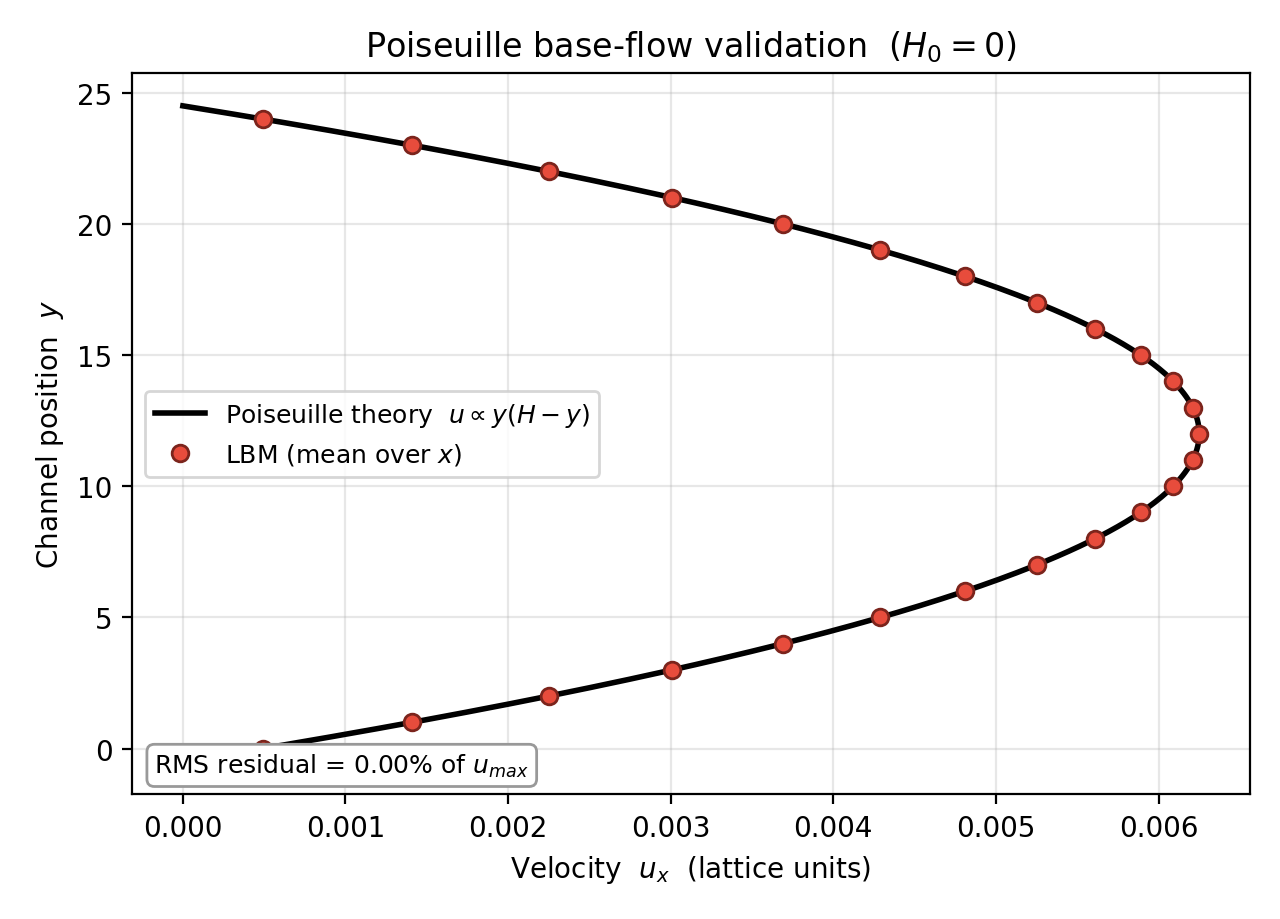
\includegraphics[width=\textwidth]{figs/poiseuille_base.png}
    \column{0.44\textwidth}
      \small
      \begin{itemize}
        \item \textbf{Setup:} a pressure-driven channel with no applied field; the LBM profile is averaged over $x$ and compared to the analytic parabola.
        \item \textbf{Result:} the profile lands on the theory with a root-mean-square residual near zero, confirming a mass- and momentum-conserving solver.
      \end{itemize}
  \end{columns}
\end{frame}

% ----------------------------- Slide 10: Validation 1 -----------------------------
\begin{frame}{Validation 1 --- Bending of Magnetic Field Lines}
  \framesubtitle{Pure magnetostatics: a magnetizable cylinder in a uniform field, flow frozen}
  \begin{columns}[T]
    \column{0.60\textwidth}
      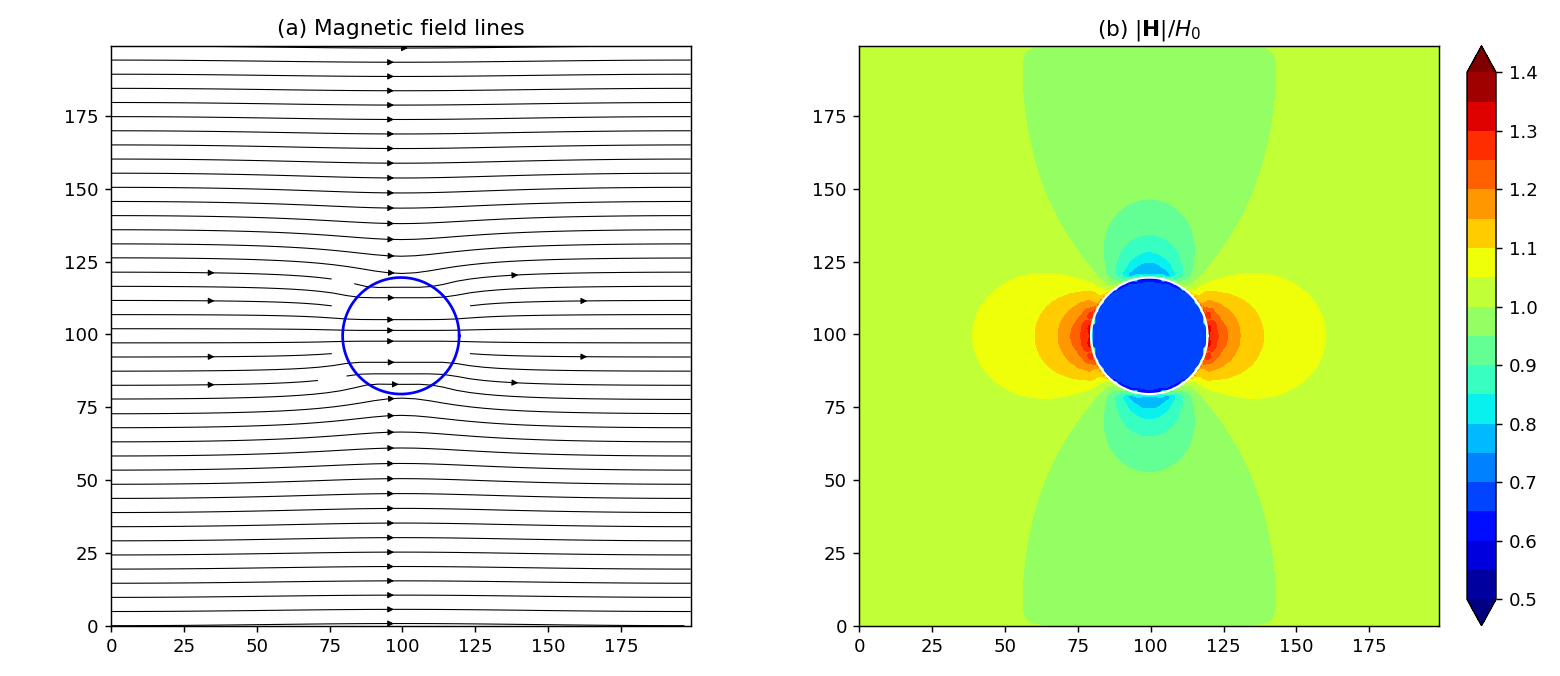
\includegraphics[width=\textwidth]{figs/val1_fieldlines.png}
    \column{0.40\textwidth}
      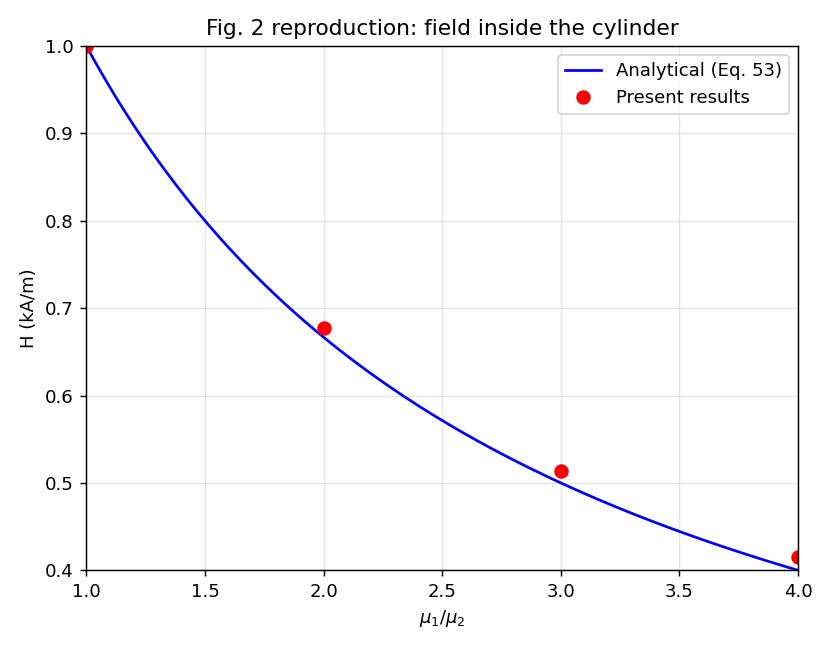
\includegraphics[width=\textwidth]{figs/val1_Hin.png}
  \end{columns}
  \vspace{0.15cm}
  \footnotesize
  \begin{itemize}
    \item \textbf{Setup:} a circular body of higher permeability in a uniform applied field, with the flow solver switched off to isolate the $h$-lattice.
    \item \textbf{Result:} the interior field matches the analytic value $H_{\text{in}}/H_0 = 2/(\mu_1/\mu_2+1)$ to within $0$--$3.8\%$ across the permeability sweep; the residual is finite-domain far-field truncation, not solver error.
    \item \textbf{Observation:} the more permeable body draws field lines into itself, giving a uniform interior field whose strength is set only by the permeability ratio.
  \end{itemize}
\end{frame}

% ----------------------------- Slide 11: Validation 2 -----------------------------
\begin{frame}{Validation 2 --- Ferrofluid Droplet Elongation}
  \framesubtitle{Coupled field, interface and flow: a droplet stretches into an ellipse}
  \begin{center}
    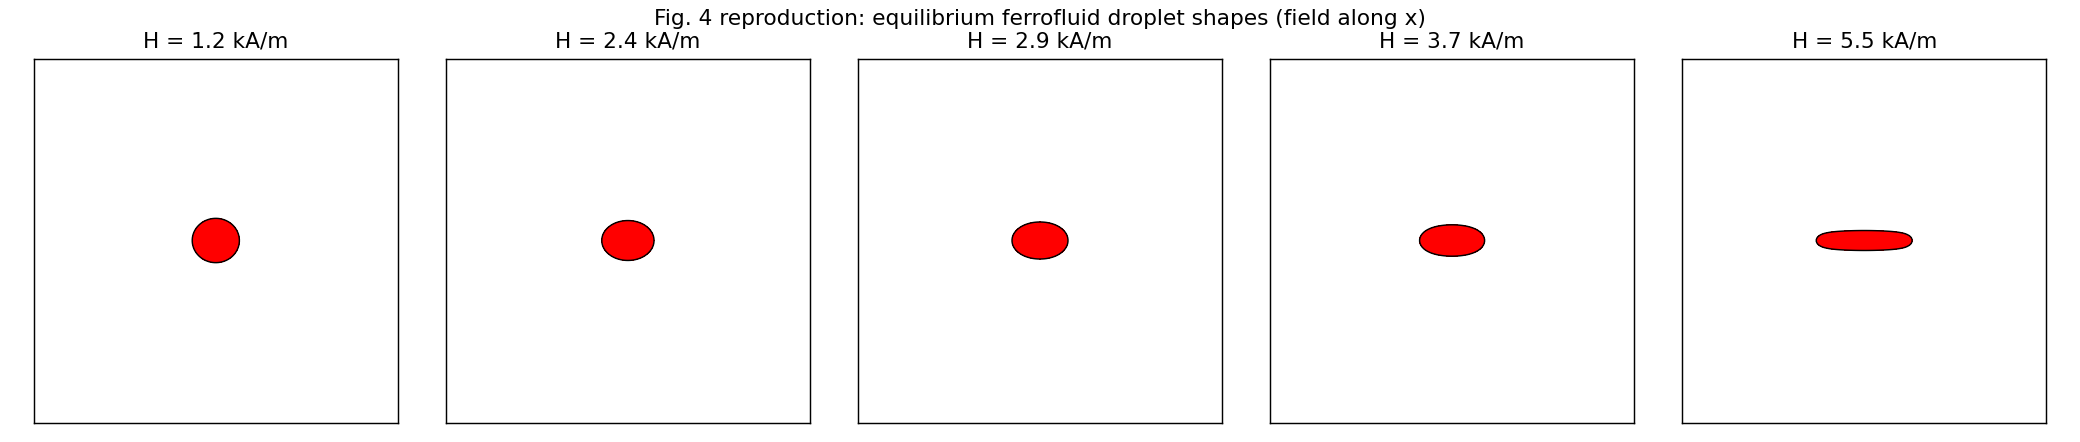
\includegraphics[width=0.92\textwidth]{figs/val2_shapes.png}
  \end{center}
  \vspace{-0.1cm}
  \begin{columns}[T]
    \column{0.5\textwidth}
      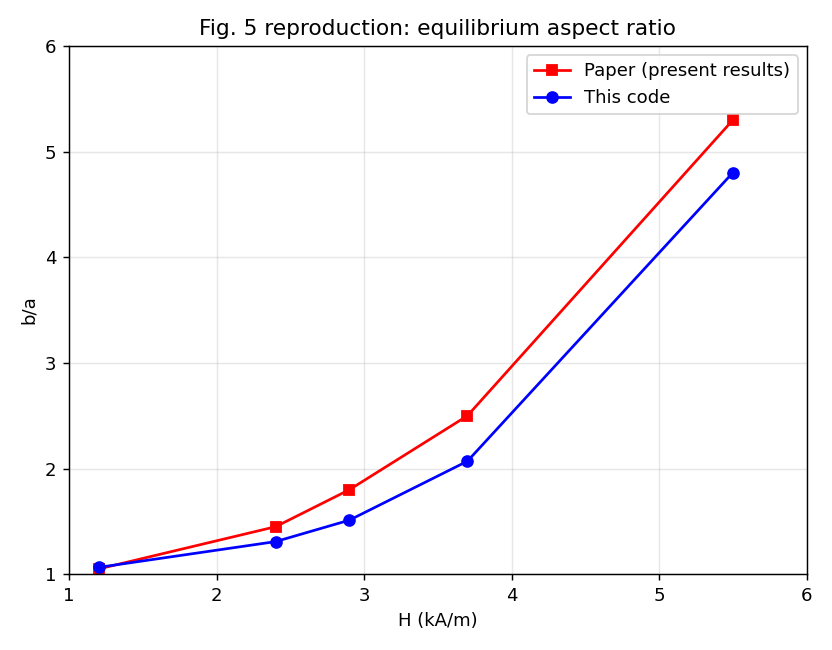
\includegraphics[width=\textwidth]{figs/val2_aspect.png}
    \column{0.5\textwidth}
      \footnotesize
      \begin{itemize}
        \item \textbf{Setup:} magnetic stress elongates the droplet along the field while surface tension resists; the aspect ratio $b/a$ is governed by the magnetic Bond number $\mathrm{Bo}_m=\chi_0^2 H^2 R/\sigma$.
        \item \textbf{Result:} the solver reproduces the reference convex $b/a(H)$ curve across the field range.
        \item \textbf{Observation:} at the two highest fields the elongated droplet wraps in the periodic-$x$ box; these points recover once the domain is enlarged.
      \end{itemize}
  \end{columns}
\end{frame}

% ----------------------------- Slide 12: Validation 3 -----------------------------
\begin{frame}{Validation 3 --- Bacri Figure 3 (central target)}
  \framesubtitle{Poiseuille flow under an oscillating field: the negative-viscosity effect}
  \begin{columns}[T]
    \column{0.62\textwidth}
      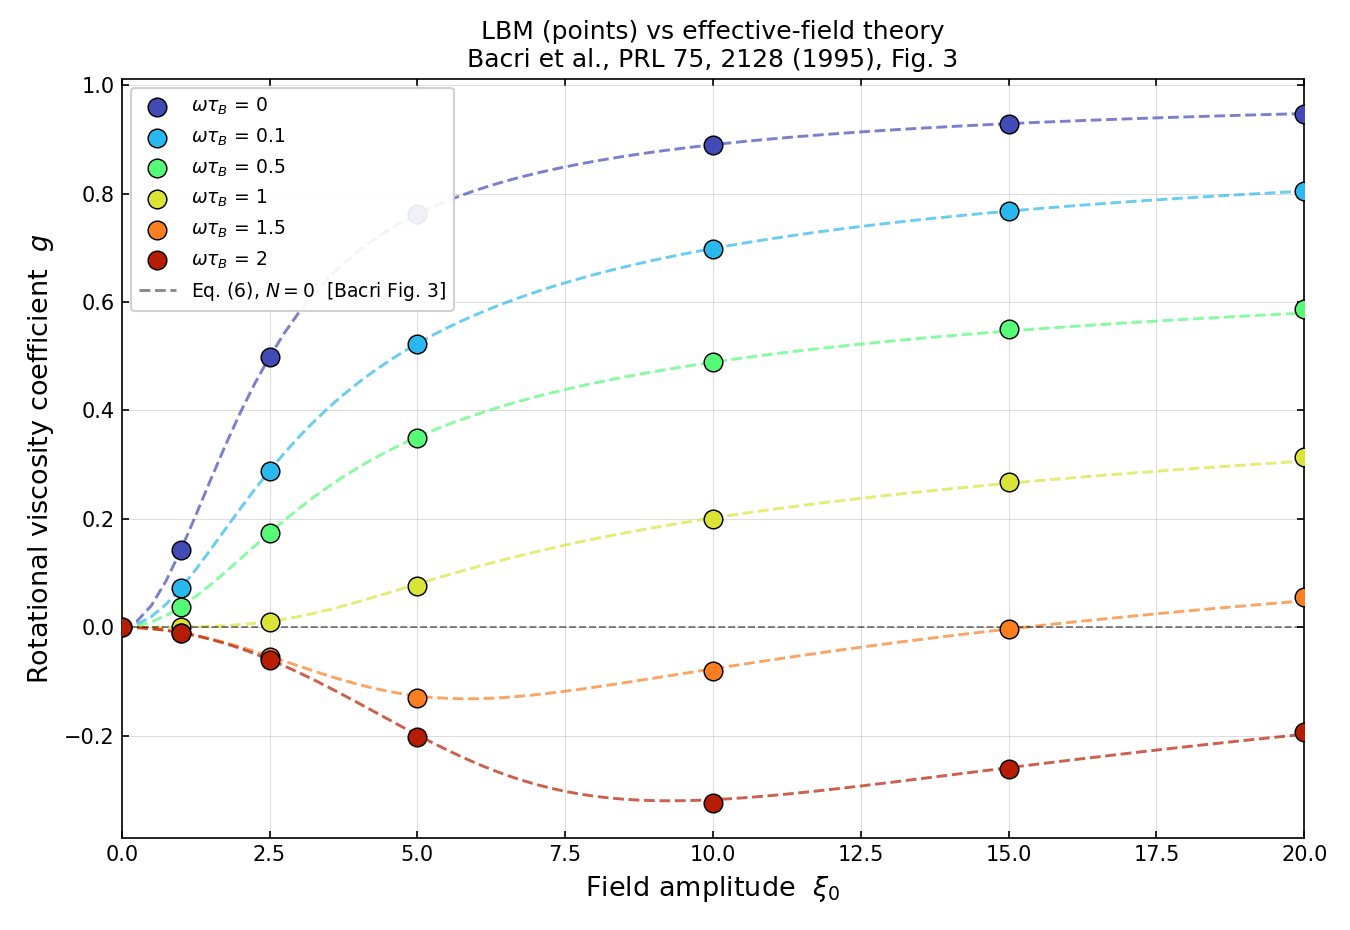
\includegraphics[width=\textwidth]{figs/val3_bacri.png}
    \column{0.38\textwidth}
      \footnotesize
      \begin{itemize}
        \item \textbf{Setup:} a body-force-driven channel flow under a linearly oscillating field; the rotational-viscosity coefficient $g(\xi_0,\omega\tau_B)$ is extracted from the converged profile.
        \item \textbf{Result:} the LBM points lie on the effective-field theory curves, with $g$ turning negative at large $\xi_0$ and high $\omega\tau_B$.
        \item \textbf{Accuracy:} $\sim 0.3\%$ in static fields; $\sim 1.6\%$ up to $\xi_0=10$, rising to $\sim 4.5\%$ at $\xi_0=20$.
      \end{itemize}
  \end{columns}
\end{frame}

% ============ Section 6 ============
\section{Purely magnetically driven flow}

% ----------------------------- Slide 13: Setup + BCs -----------------------------
\begin{frame}{Purely Magnetically Driven Flow --- Setup}
  \framesubtitle{Field formulation, driving mechanism, and boundary conditions}
  \begin{columns}[T]
    \column{0.53\textwidth}
    \small
    \begin{itemize}
      \item \textbf{Formulation:} a harmonic, centreline-symmetric applied potential,
      \[ A_{\text{app}}=\mu_0(H_d\,Y+k\,XY), \]
      \[ \bm H_{\text{app}}=(H_d+kX,\,-kY). \]
      \item \textbf{Mechanism:} the streamwise Kelvin force $F_{K,x}\approx\mu_0 M(H_d)\,k$ replaces the pressure gradient. A non-zero $H_d$ is required, since a pure-gradient field has a null at the centre and gives no net drive.
      \item \textbf{Values:} $H_d=1.73$, $k=1.21\times10^{-5}$ (matched to $G=2\times10^{-7}$).
    \end{itemize}
    \column{0.47\textwidth}
    \centering
    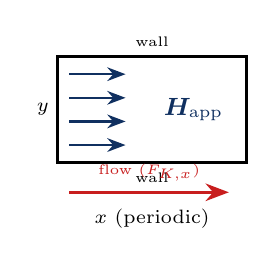
\begin{tikzpicture}[>=Stealth,scale=0.75]
      \draw[very thick] (0,0) rectangle (3.2,1.8);
      \node at (1.6,2.05){\tiny wall};
      \node at (1.6,-0.25){\tiny wall};
      \foreach \y in {0.3,0.7,1.1,1.5}{
        \draw[->,iitblue,thick] (0.2,\y) -- (1.15,\y);}
      \node[iitblue] at (2.3,0.9){\small $\bm H_{\text{app}}$};
      \draw[->,iitred,very thick] (0.2,-0.5) -- (2.9,-0.5) node[midway,above]{\tiny flow ($F_{K,x}$)};
      \node at (-0.25,0.9){\scriptsize $y$};
      \node at (1.6,-0.95){\scriptsize $x$ (periodic)};
    \end{tikzpicture}

    \vspace{0.35cm}
    \raggedright\footnotesize
    \textbf{Boundary conditions}
    \begin{itemize}\footnotesize
      \item Walls ($f,g$): no-slip via halfway bounce-back.
      \item Walls ($h$): Neumann on $A_z$, $\partial A_z/\partial n=\mu_0(\bm H_{\text{app}}+\bm M_w)\cdot\hat{\bm t}$.
      \item $x$: periodic; jump-periodic seam on $A_z$ ($A_{\text{app}}$ is not periodic).
      \item Single-phase runs ($\phi\equiv 1$).
    \end{itemize}
  \end{columns}
\end{frame}

% ----------------------------- Slide 14: transverse balance -----------------------------
\begin{frame}{The Transverse Force Balance ($y$-direction)}
  \framesubtitle{Confirming the setup stays unidirectional and fully developed}
  \footnotesize
  \textbf{Purpose:} verify the assumption behind the boundary conditions --- that the transverse force does not disturb the channel flow.
  \begin{center}
    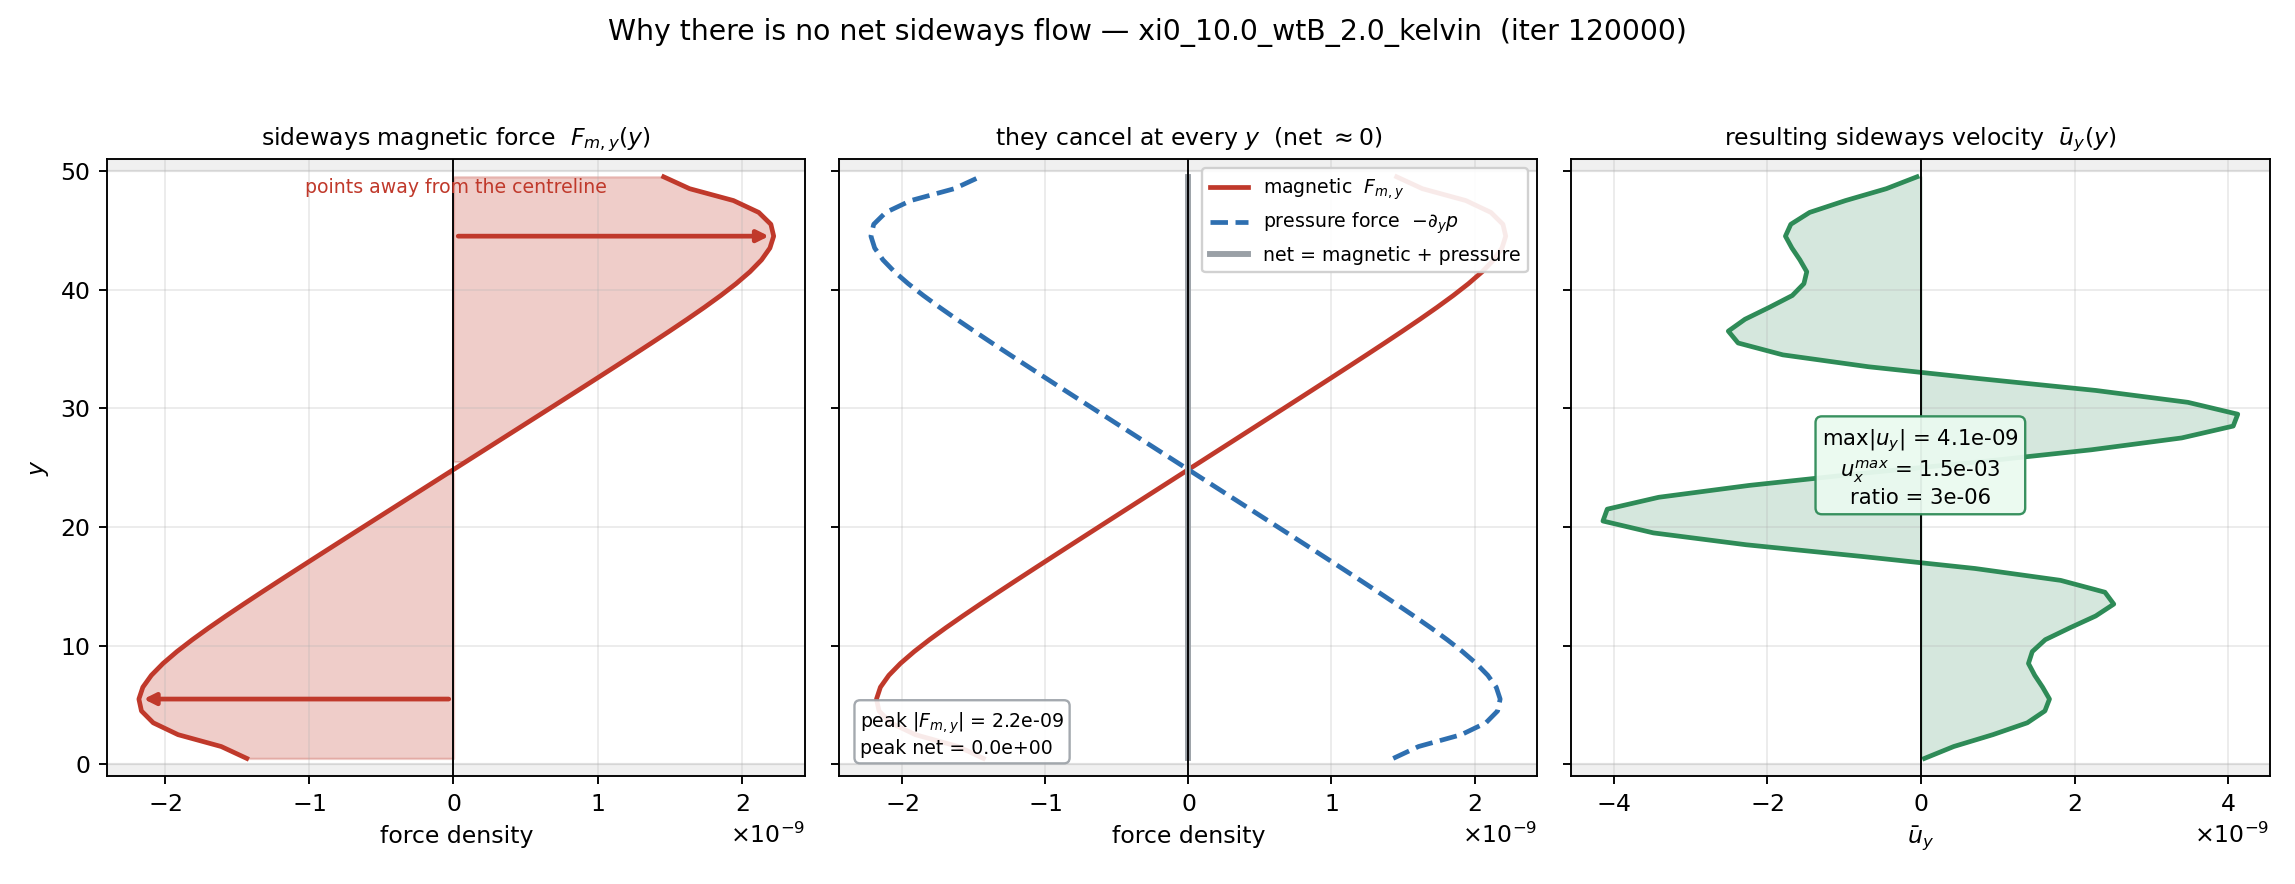
\includegraphics[width=0.88\textwidth]{figs/mag_ybalance.png}
  \end{center}
  \vspace{-0.1cm}
  \footnotesize
  \begin{itemize}
    \item \textbf{Observation:} at every height the transverse magnetic force $F_{m,y}$ (red) is cancelled by the pressure force (blue); the net transverse velocity is $|u_y|\sim10^{-9}$ against $u_x^{\max}\sim10^{-3}$.
    \item \textbf{Mechanism:} $F_{m,y}$ depends on $y$ alone, so it is a pure gradient that pressure absorbs exactly. Only the mean streamwise force survives, because periodicity prevents pressure from developing a mean slope along $x$.
  \end{itemize}
\end{frame}

% ----------------------------- Slide 15: velocity profile -----------------------------
\begin{frame}{Velocity Profile under Purely Magnetic Drive}
  \begin{columns}[T]
    \column{0.56\textwidth}
      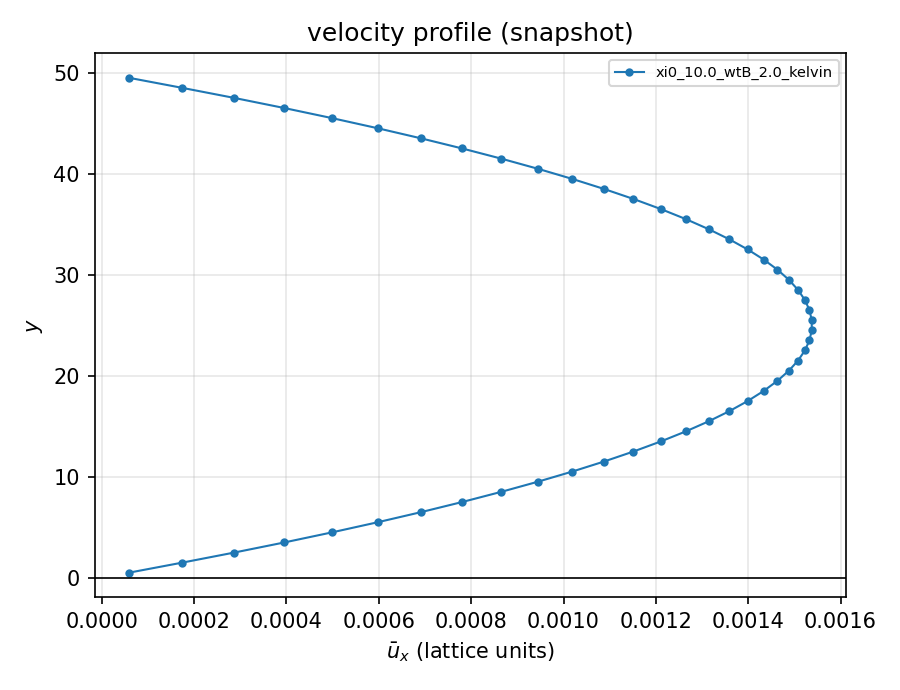
\includegraphics[width=\textwidth]{figs/mag_profile.png}
    \column{0.44\textwidth}
      \begin{itemize}
        \item \textbf{Result:} the field alone produces a clean parabolic profile with $u_x^{\max}\approx1.5\times10^{-3}$.
        \item \textbf{Observation:} the transverse force leaves no imprint on the profile; no secondary circulation appears.
        \item \textbf{Implication:} a spatially graded magnetic field reproduces textbook Poiseuille flow, demonstrating a valveless magnetic pump.
      \end{itemize}
  \end{columns}
\end{frame}

% ----------------------------- Slide 16: Bacri Fig 3 equivalent -----------------------------
\begin{frame}{Negative Viscosity under Magnetic Drive}
  \framesubtitle{The Bacri Figure 3 equivalent for the purely Kelvin-driven flow}
  \begin{columns}[T]
    \column{0.56\textwidth}
      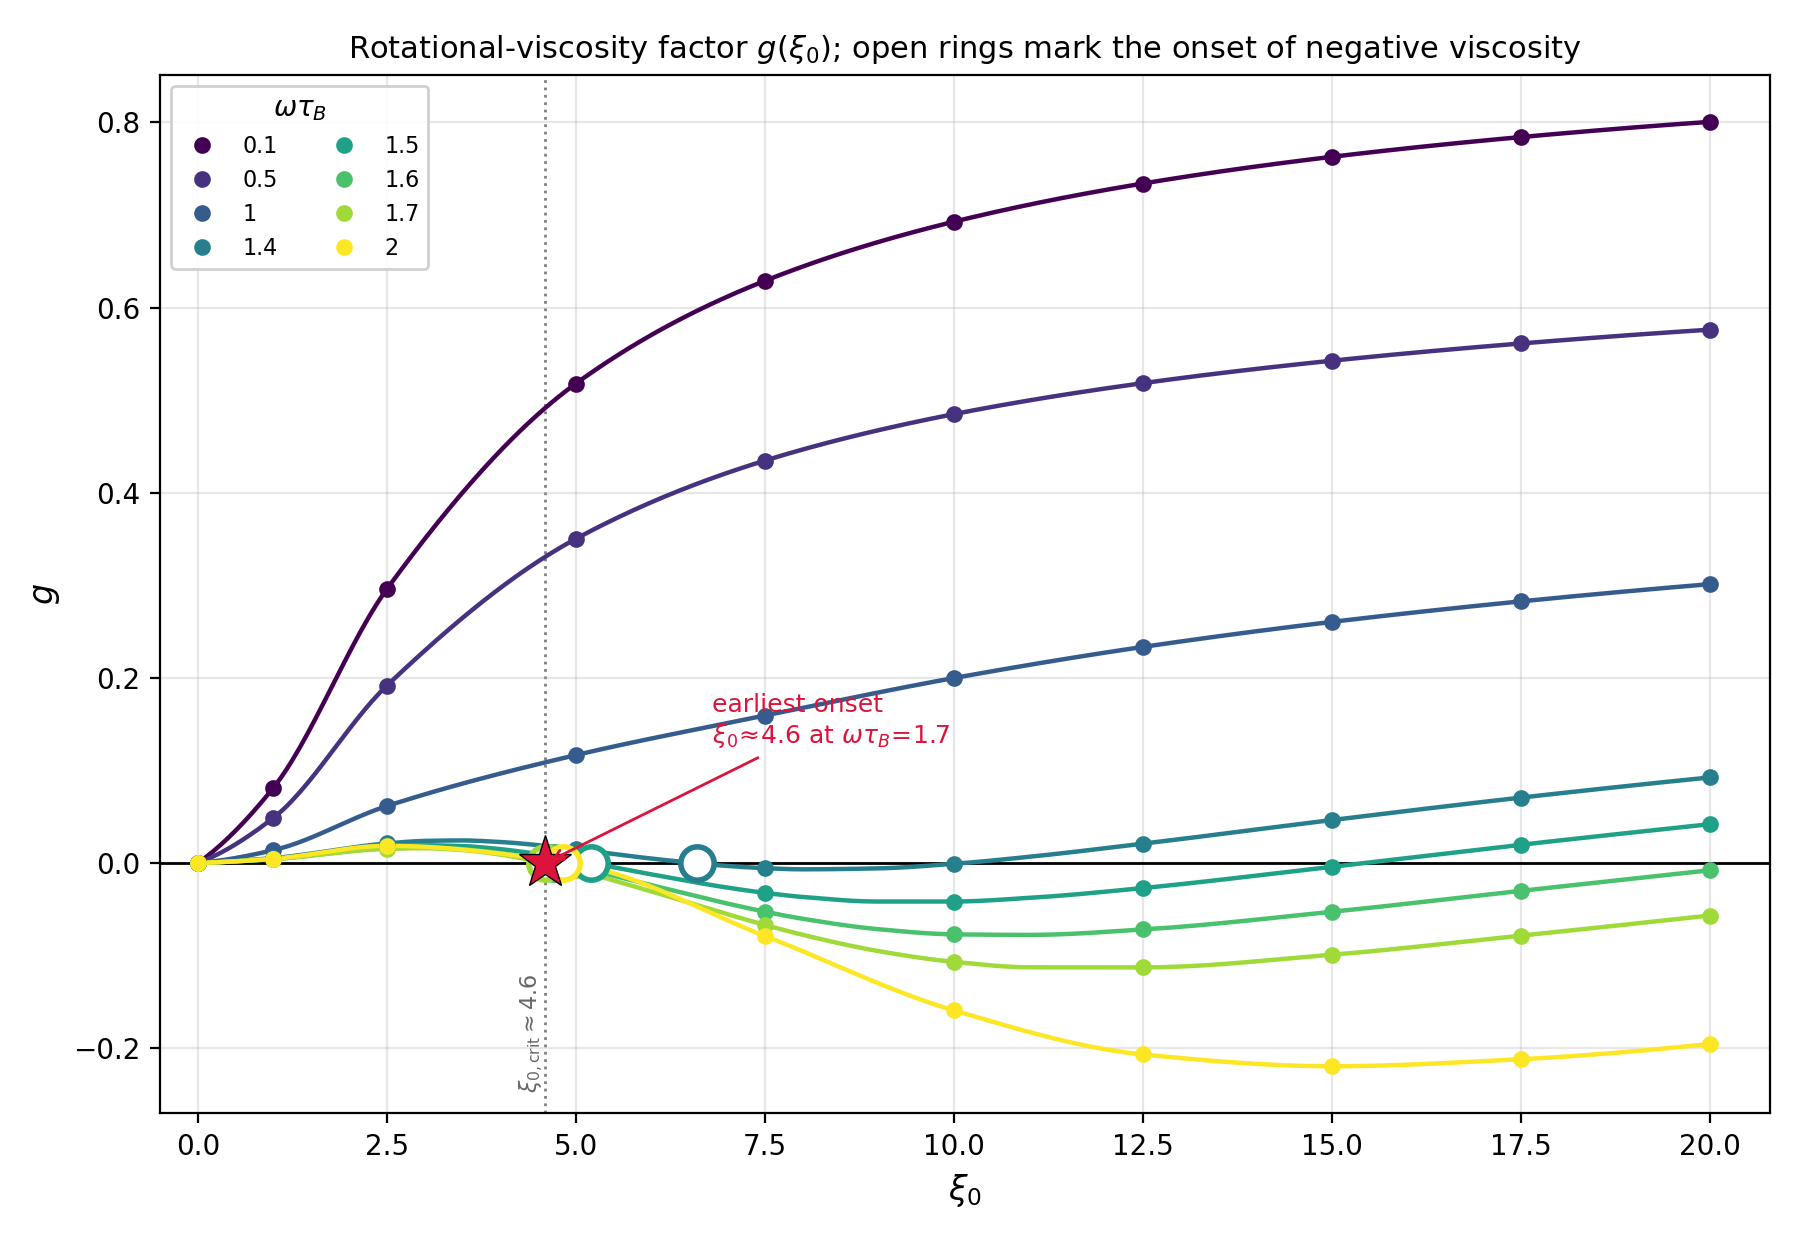
\includegraphics[width=\textwidth]{figs/mag_onset.png}
    \column{0.44\textwidth}
      \footnotesize
      \begin{itemize}
        \item \textbf{Persistence:} the effect survives with \emph{zero} external pressure gradient; the same field both pumps and modulates the flow.
        \item \textbf{Threshold:} viscosity stays positive until $\xi_0\approx4.6$, beyond which $g$ turns negative.
        \item \textbf{Optimal drive:} onset is reached at the smallest field near $\omega\tau_B\approx1.7$.
      \end{itemize}
  \end{columns}
\end{frame}

% ============ Section 7 ============
\section{Outlook}

% ----------------------------- Slide 17: Future work -----------------------------
\begin{frame}{Future Work}
  \begin{itemize}
    \item \textbf{Coupled oscillating shear and field:} the change in apparent viscosity when the fluid is subjected to both an oscillating shear and an oscillatory magnetic field at the same frequency $\omega$.
    \item \textbf{Full two-phase Kelvin-driven flow:} couple the water/ferrofluid interface to the purely magnetically driven configuration.
    \item \textbf{Thermal coupling:} add the energy equation for temperature-dependent magnetization and thermomagnetic convection.
    \item \textbf{Antisymmetric-field pumping:} directional flow generated by specially tailored antisymmetric oscillating fields.
    \item \textbf{Three-dimensional extension:} generalize the vector-potential formulation beyond the planar channel.
  \end{itemize}
\end{frame}

% ----------------------------- Slide 18: References & acknowledgments -----------------------------
\begin{frame}{References \& Acknowledgments}
  \small
  \textbf{References}
  \begin{enumerate}
    \item Shliomis, M.~I. (2002). Effective viscosity of magnetic fluids. \emph{Physical Review E}, \textbf{64}(6).
    \item Bacri, J.-C., \& Perzynski, R. (1995). ``Negative-Viscosity'' Effect in a Magnetic Fluid. \emph{Physical Review Letters}, \textbf{75}(11).
    \item Hu, Y., \& Li, D. (2018). Phase-field-based lattice Boltzmann model for multiphase ferrofluid flows. \emph{Physical Review E}, \textbf{98}, 033301.
  \end{enumerate}
  \vspace{0.4cm}
  \textbf{Acknowledgments}\\[3pt]
  I sincerely thank my supervisor, Prof.\ Jayati Sarkar, for her guidance throughout this work, and the Department of Chemical Engineering, IIT Delhi, for its support.
\end{frame}

% ----------------------------- Slide 19: Thank You -----------------------------
\begin{frame}[plain]
  \vfill
  \begin{center}
    
\includegraphics[height=1.9cm]{figs/iitd_logo.png}\\[0.8cm]
    {\Huge\bfseries Thank You}
  \end{center}
  \vfill
\end{frame}

\end{document}
